\graphicspath{ {Figures/chapter04} }
In this chapter we will focus on designing an appropriate controller theoretically and experimentally 
\section{System Requirements}
Before starting into the evaluation of the controller's performance, certain requirements conditions and specifications have been identified as crucial benchmarks. These prerequisites provide a foundational base  to be able to determine if the controller performs well enough:

\begin{enumerate}
\item the plate to incline only in \(15\deg\) in both coordinates.
\item Settling time less than 5 seconds (\(Ts < 5\))
\item Rise time less or equal to 1 seconds (\(T_r < 0.5\)).
\item A overshoot less than 20\% (\(M < 0.20\)).
\item The static error should be equal to zero or less than 25 pixels (\(e_0 < 0.05\)).
\end{enumerate}
The goal is that the controller will be able to fulfill these demands.

\section{System Controllability and Observerability}
The controllability and observability of the system are crucial aspects in ensuring effective control. In order to have full freedom in the placement of the poles, it is necessary to check the controllability of the system. This is done by determining the controllability matrix $S$ \cite{nise2020control}, which is given by:
\begin{equation}
S = \begin{bmatrix}
B & AB & A^2B & \dots & A^{n-1}B
\end{bmatrix}
\end{equation}
where $n$ is the number of states. If the determinant of the matrix $S$ is non-zero, it indicates that the placement of the poles is not restricted, allowing for the fulfillment of control demands.
Using the overall plant transfer function in Eq. (3.48), The determined controllability matrix:
\begin{equation}
   S = 1.0 \times 10^5 \times
    \begin{bmatrix}
        0 & 0 & 0 & -0.0158 \\
        0 & 0 & -0.0158 & 0.3527 \\
        0 & 0.0023 & 0.0010 & 0.6159 \\
        0.0023 & -0.0503 & 0.6159 & -2.4073 \\
    \end{bmatrix} 
\end{equation}
The rank of the controllability matrix Eq.(4.2) for the linear model is 4, which is full rank meaning the system is completely controllable


Observability is equally important, as the controller needs to have all the information to control the system successfully. The observability of the system can be checked using the observability matrix $O$, defined as:
\begin{equation}
   O = 
\begin{bmatrix}
    C \\
    CA \\
    CA^2 \\
    \vdots \\
    CA^{n-1}
\end{bmatrix}
\end{equation}

Just like in controllability, if the observability matrix Eq.(4.4) is full rank then the system is observable.
\begin{equation}
   O = 
\begin{bmatrix}
    1.0000 & 0 & 0 & 0 \\
    0 & 1.0000 & 0 & 0 \\
    0 & 0 & -7.0071 & 0 \\
    0 & 0 & 0 & -7.0071 \\
\end{bmatrix}
\end{equation}
Since the matrix O is full rank (rank(O) = 4). This
means that we can estimate all the states from the displacement measurement and the system is both observable and controllable

\section{PID Controller design}
The Proportional Integral Derivative (PID) controller is one of the most widely used controllers today. The ideal PID controller is described by the equation:
\begin{equation}
u(t) = K_P e(t) + K_I \int_0^t e(\tau) d\tau + K_D \frac{d}{dt} e(t)
\end{equation}
where \(u\) represents the control signal and \(K_p\) , \(K_I\) and \(K_D\) denote the proportional, integral and derivative gains respectively. Notably large value for \(K_p\) leads to increased speed of the controller. However, it can compromise stability. \(K_I\) 
eliminates static error, but also decreases stability. On the other hand the derivative gain, \(K_D\), decreases the oscillation and leads to stability enhancement 
The closed-loop transfer function of a PID-controlled system is given by: Eq.4.2 where s is the Laplace variable
\begin{equation}
G_c(s) = K_P + \frac{K_I}{s} + K_Ds 
\end{equation}
To enable the PID controller's operation, the error \(e(t)\) is essential. This error is derived by taking the difference between the reference signal \(r(t)\) and the actual system output \(x(t)\)), represented as the variance between the desired position  and the sensed position (as depicted in Fig. 4.1). In this illustration, two feedback loops are evident. The internal loop corresponds to the servomotor's internal controller, managing its own dynamics. Simultaneously,  and the external loop ensures that the PID controller receives the necessary input after error calculation
\begin{figure}[h]
    \centering
    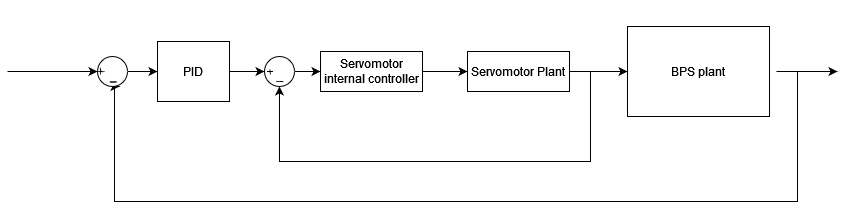
\includegraphics[width=0.95\linewidth]{PID_digram.png}
    \caption{A block diagram illustrates BPS's control mechanism using PID}
    
\end{figure}

In real-world scenarios, achieving an optimal PID controller often involves considering the inherent dynamics and characteristics of the system. Practical tuning methods, such as frequency response analysis or model-based approaches, provide engineers with tools to fine-tune the controller parameters for specific performance criteria. In order to meet our requirements, we utilized the Simulink PID block tuner tool. The block diagram, as depicted in Fig. 4.2, served as the foundation for our tuning process.

\begin{figure}[h]
    \centering
    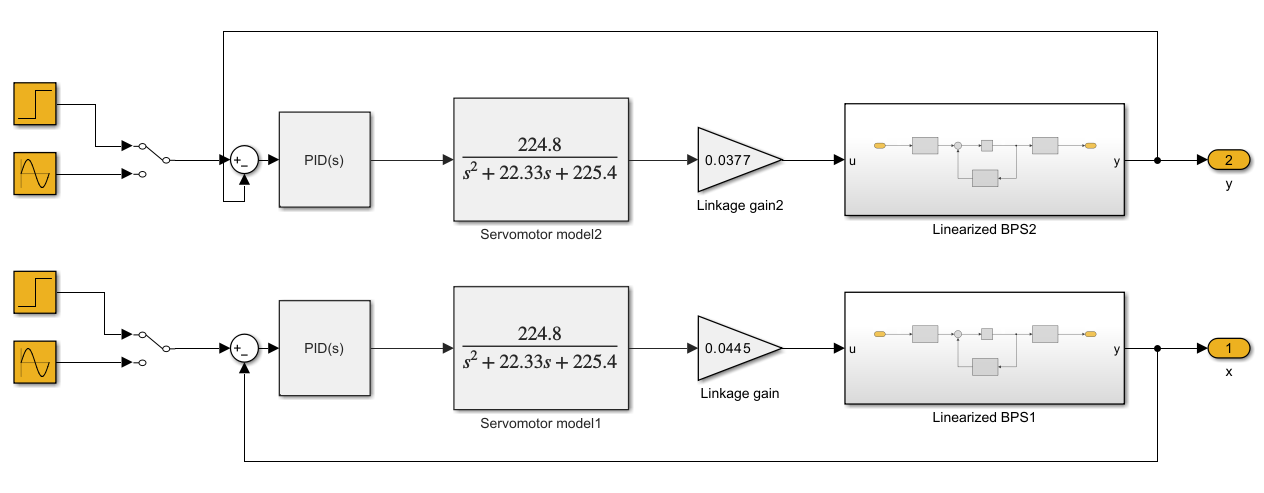
\includegraphics[width=0.95\linewidth]{idealPID.png}
    \caption{the simplified Simulink PID diagram, highlighting its key components and signal pathways}
    
\end{figure}

Although our tuning efforts using the Simulink PID block tuner tool yielded a very good response, we faced some challenges that required attention. The main concern was the PID output,  went beyond the 0 to 180-degree range. This presented a practical issue as the servo couldn't handle values outside its normal operational limits.

Moreover, our sensor provided the ball position through an analog signal ranging from 0 to 1024, making it necessary to make adjustments to the model. To resolve these issues, we implemented a saturation function to limit the PID output within a manageable range. Additionally, we introduced a calibration transformation and filter to the sensor signal. To account for calculation and data transmission delays, we incorporated a delay component into the model.

These adjustments and refinements led us to the development of Fig. 4.3, which represents a more practical and realistic model (a higher quality image can be found in appendix B). This modified model takes into account the limitations and characteristics of both the servo and the sensor and considers the calculation and data transport delay from the computer to the arduino and vice versa.

\begin{figure}
    \centering
    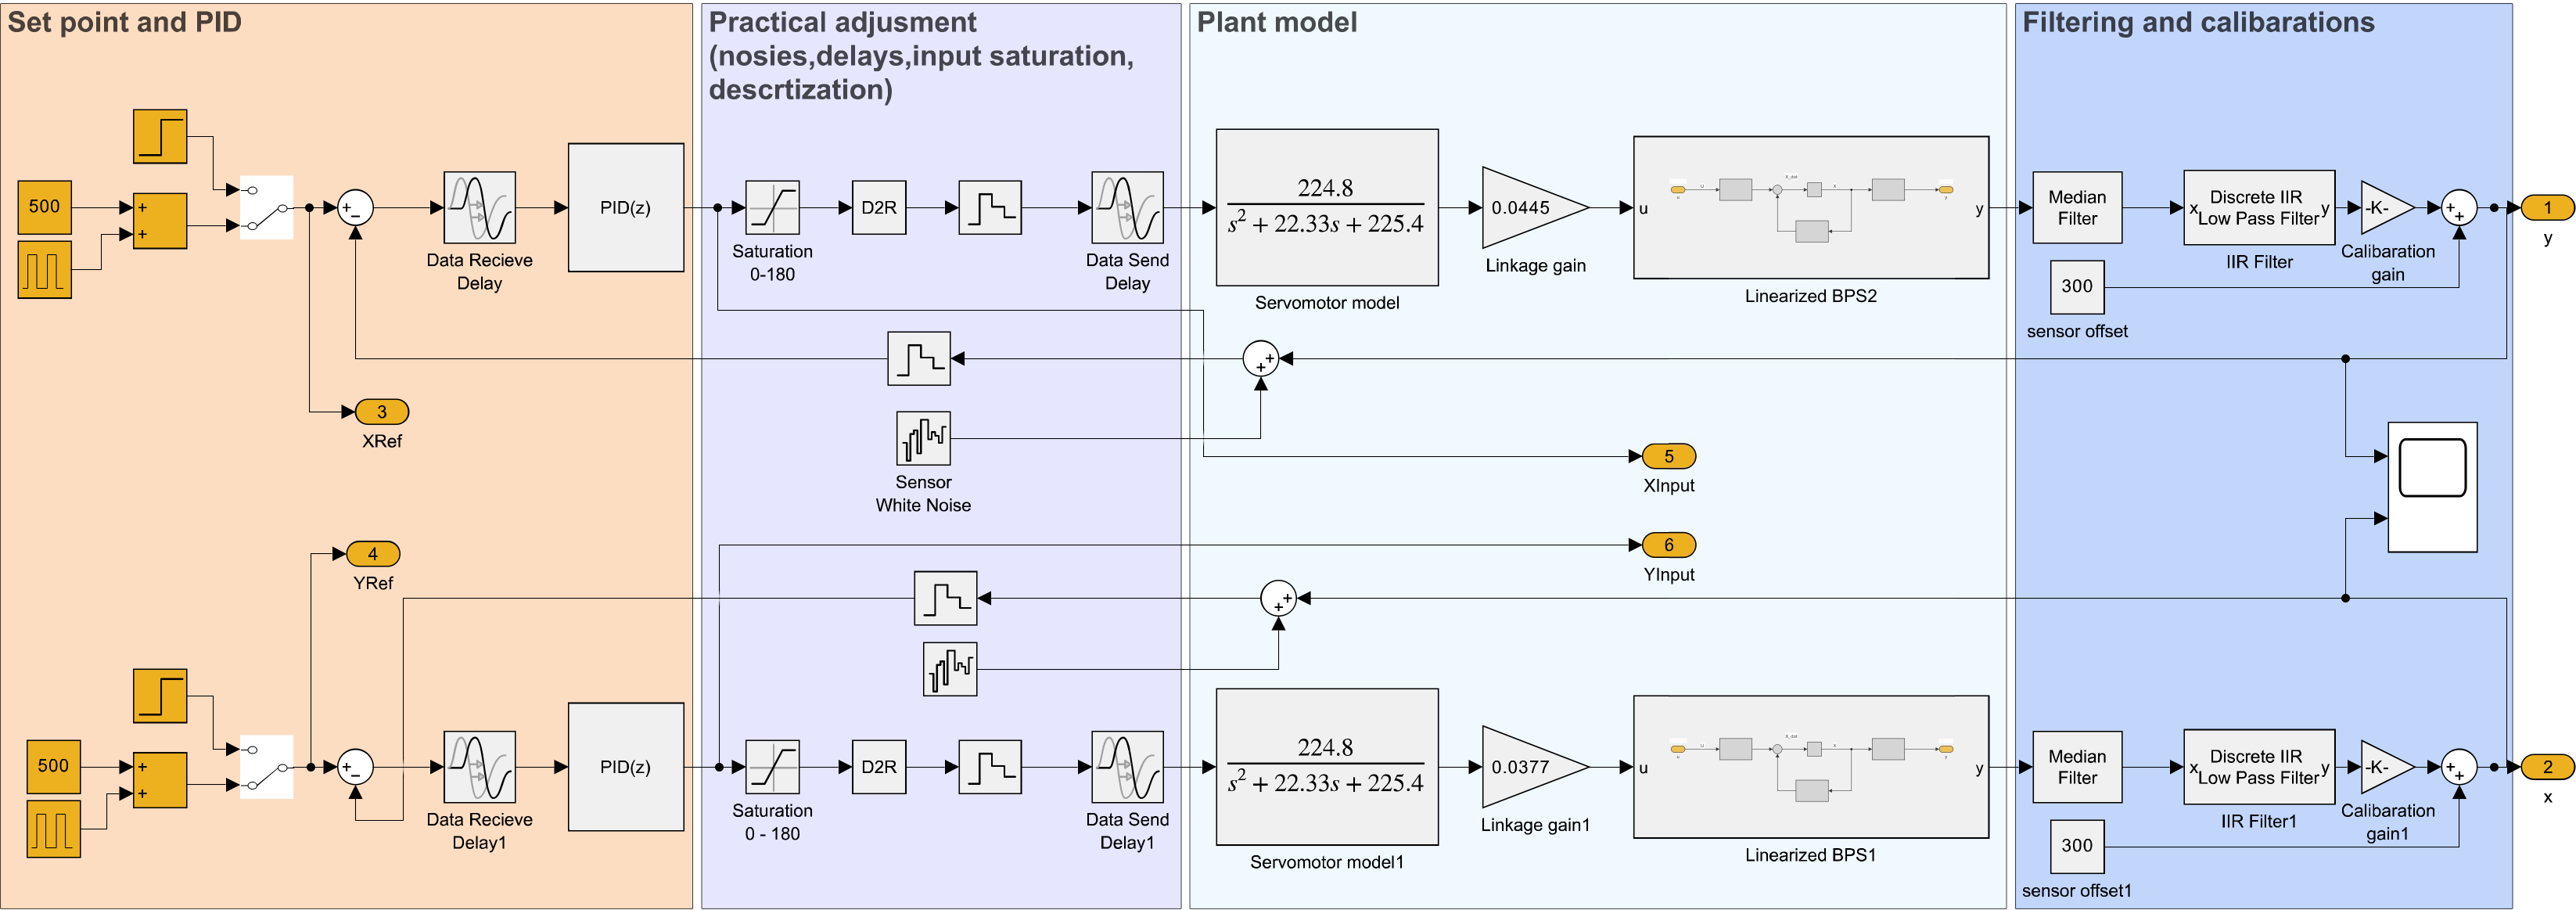
\includegraphics[width=1\textwidth]{practicalPID.png}
    \caption{Refined Simulink Model Illustrating Practical Adjustments}
    
\end{figure}
As a result of these adjustments introduced complexity and non-linearity to the system that surpassed the capabilities of SIMULINK tuning tools. Consequently, we shifted to a manual tuning approach, relying on a trial-and-error method to iteratively fine-tune the parameters for optimal system performance. 
The PID gains, determined through manual tuning using a trial-and-error method, are summarized in Table 1.

\begin{table}[h]
    \centering
    \caption{Tuned PID Parameters}
    
    \begin{tabular}{|c|c|c|c|}
        \hline
        &
        \text{Proportional Gain (\(K_P\))} & 
        \text{Integral Gain (\(K_I\))} & 
        \text{Derivative Gain (\(K_D\))} \\
        \hline
        \hline
        PID X 1 & 
        \text{0.125} &
        \text{0.00184} & 
        \text{0.098} \\
        \hline
        PID Y 1 & 
        \text{0.127} &
        \text{0.00084} & 
        \text{0.088} \\
        \hline
        \hline
        PID X 2 & 
        \text{0.165} &
        \text{0.00085} & 
        \text{0.11} \\
        \hline
        PID Y 2 & 
        \text{0.167} &
        \text{0.00084} & 
        \text{0.105} \\
        \hline
        \hline
        PID X 3 & 
        \text{0.105} &
        \text{0.00084} & 
        \text{0.07} \\
        \hline
        PID Y 3 & 
        \text{0.107} &
        \text{0.00184} & 
        \text{0.069} \\
        \hline
        \hline
    \end{tabular}
\end{table}


\section{PID Controller Implementation}
After the theoretical foundation of the PID controller design, the next crucial step is its practical implementation. This section outlines the real-world application of the PID controller to control the Ball and Plate System (BPS).

\subsection{Real System Implementation}

The PID controller, designed based on the principles discussed earlier, was implemented in the physical BPS. Figure 4.4 showcases the real system setup, highlighting the integration of the PID controller into the overall system.

\begin{figure}[h]
    \centering
    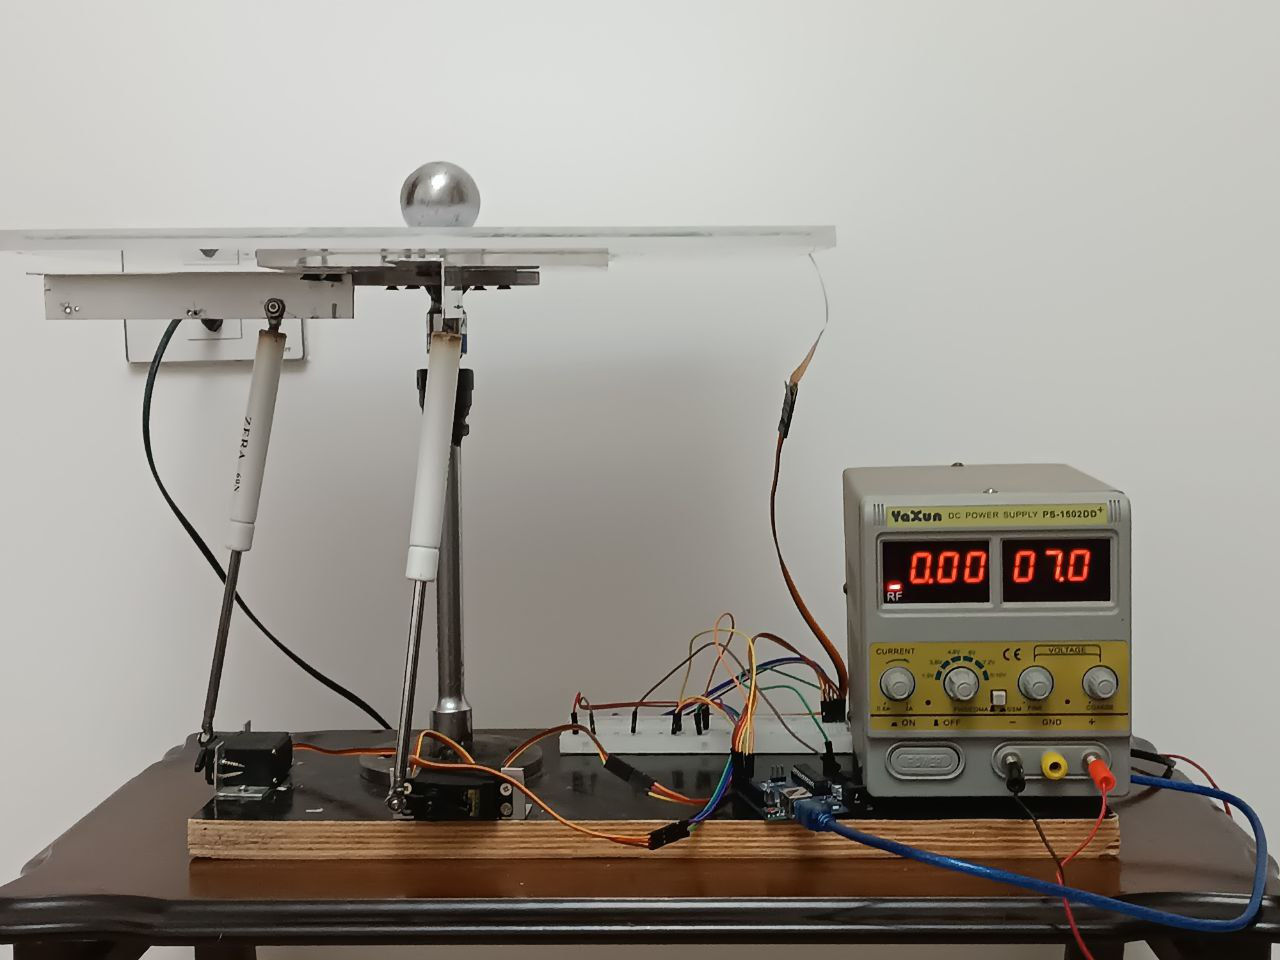
\includegraphics[width=0.95\linewidth]{real_plant.jpg}
    \caption{Real System Implementation with PID Controller}
    \label{fig:real-system-implementation}
\end{figure}

In this configuration, the PID controller interacts with the servomotors to adjust the position of the plate in response to the sensed ball position. The physical setup involves the Arduino Uno, servomotors, resistive touch screen, and the mechanical structure of the BPS.

\subsection{Simulink Model for PID Control}

To facilitate a seamless interaction between the PID controller and the real system, a Simulink model was developed. Figure 4.5 illustrates the Simulink model responsible for PID control (a higher quality image can be found in appendix B), incorporating the practical adjustments discussed earlier.

\begin{figure}[h]
    \centering
    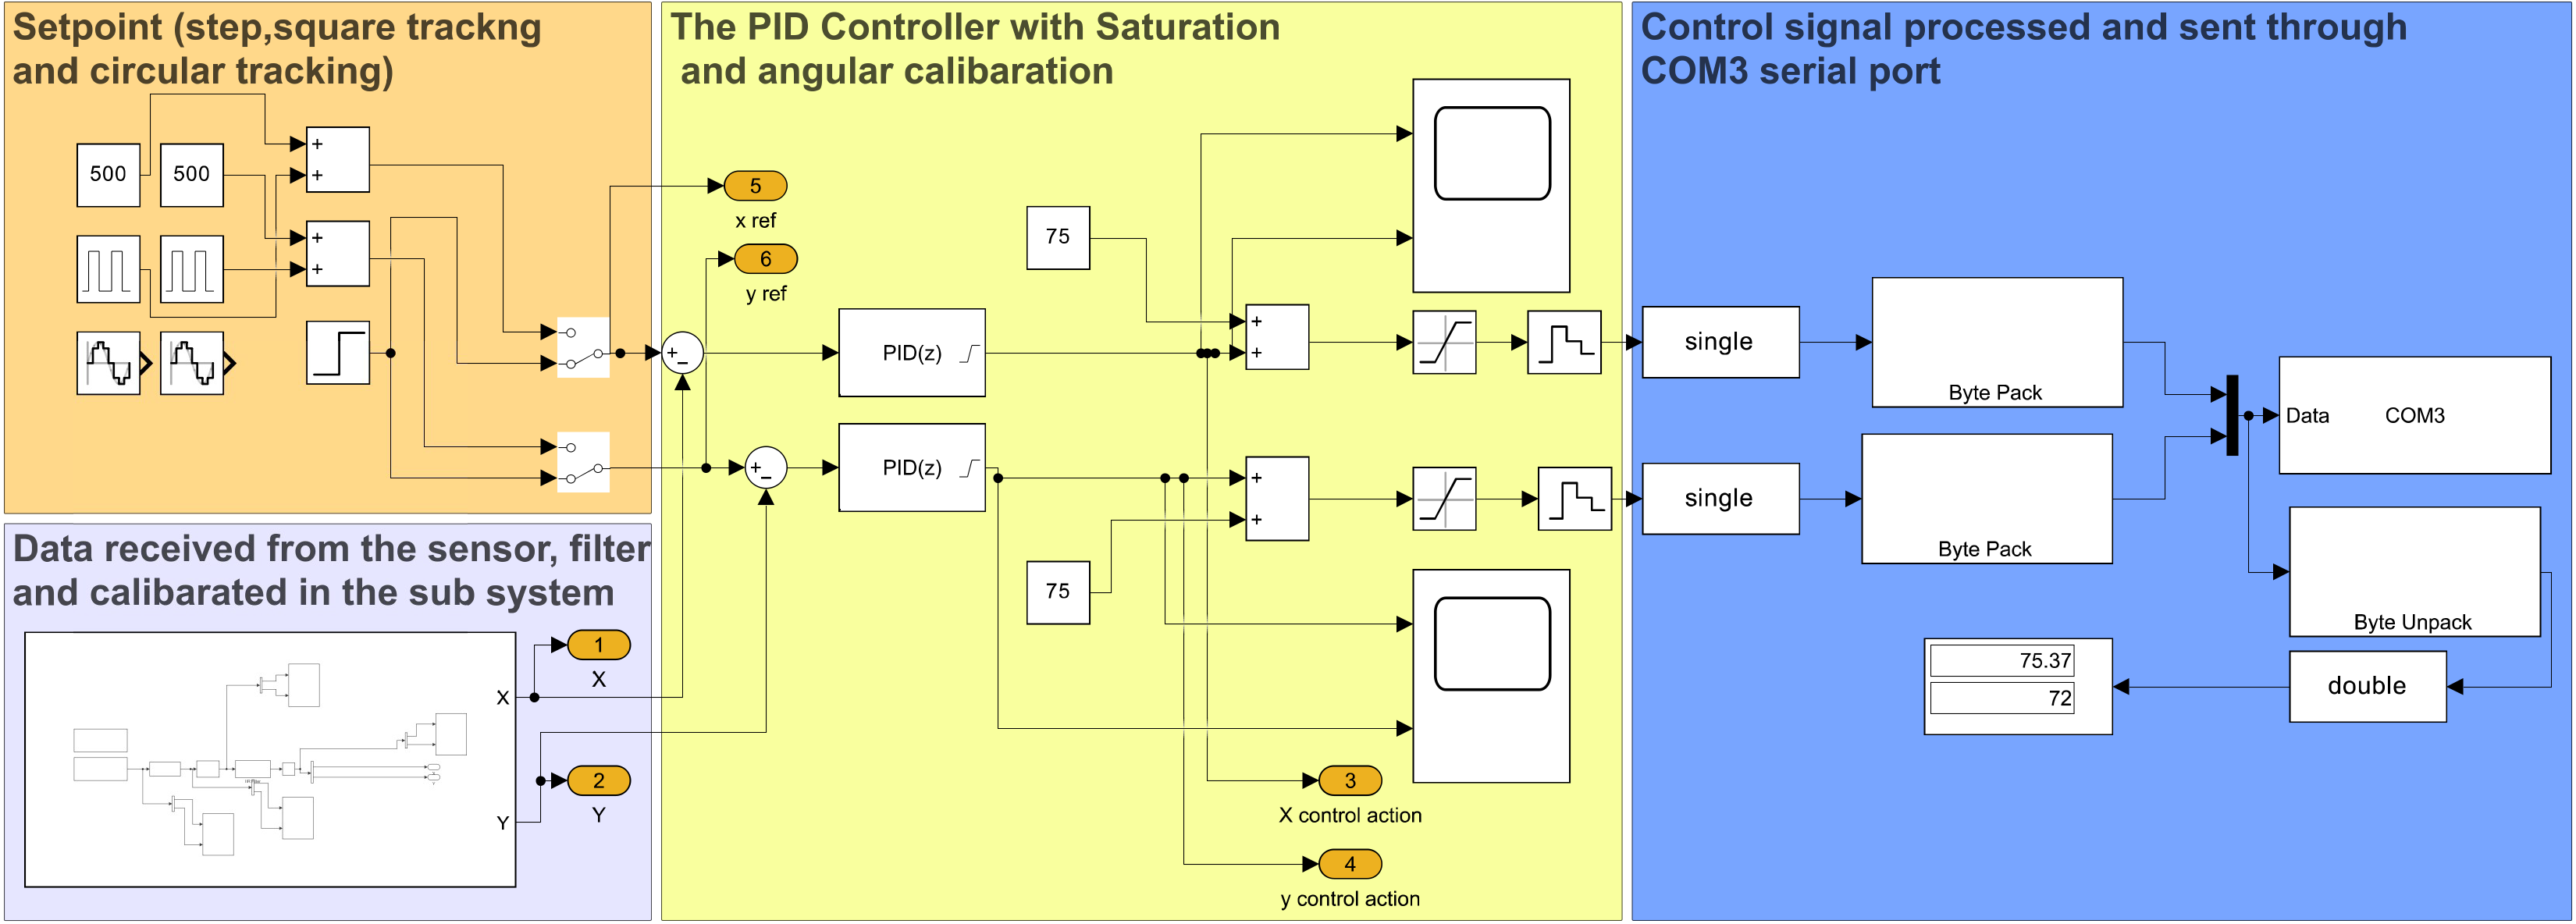
\includegraphics[width=0.95\linewidth]{simulink_real_system_pid_model.png}
    \caption{Simulink Model for PID Control Implementation}
    \label{fig:simulink-pid-model}
\end{figure}

The Simulink model integrates the PID block with the plant model, representing the dynamics of the BPS. Additionally, it includes the saturation function, calibration transformation, and filters to ensure compatibility with the real-world limitations of the servo and sensor.

The communication between the Simulink model and the real system is established through the Arduino via COM3 serial pot, which serves as the intermediary for data exchange. This bidirectional communication allows the Simulink model to receive real-time data from the system and send control signals back for continuous adjustment.

\subsection{Challenges and Manual Tuning}

Despite the theoretical foundation and simulation-based tuning, the real-world implementation presented challenges. 

One of the initial challenges was determining the appropriate time sampling for the PID controller to ensure compatibility with the Arduino. An approximate time sample for the Arduino was estimated, considering its processing capabilities, and additional delay factors were incorporated. After an iterative experimentation, it became evident that a time sample of 0.08 seconds provided the best response.the chosen time sampling is crucial for the overall responsiveness of the PID controller in the real system. It plays a pivotal role in balancing the need for rapid adjustments with the Arduino's processing constraints. This optimization contributes to achieving a smooth and stable control mechanism for the Ball and Plate System.
\begin{onehalfspacing}
Another significant challenge encountered during the real-time implementation was associated with the differential part of the PID controller. In instances where the ball experienced sudden and significant movements, resulting in rapid changes in its position, the differential component of the controller exhibited a behavior known as "differential kicks" presented in Fig. 4.6. These sudden kicks or spikes in Fig. 4.6 had a detrimental impact on the stability of the ball on the plate.


\begin{figure}[h]
    \centering
    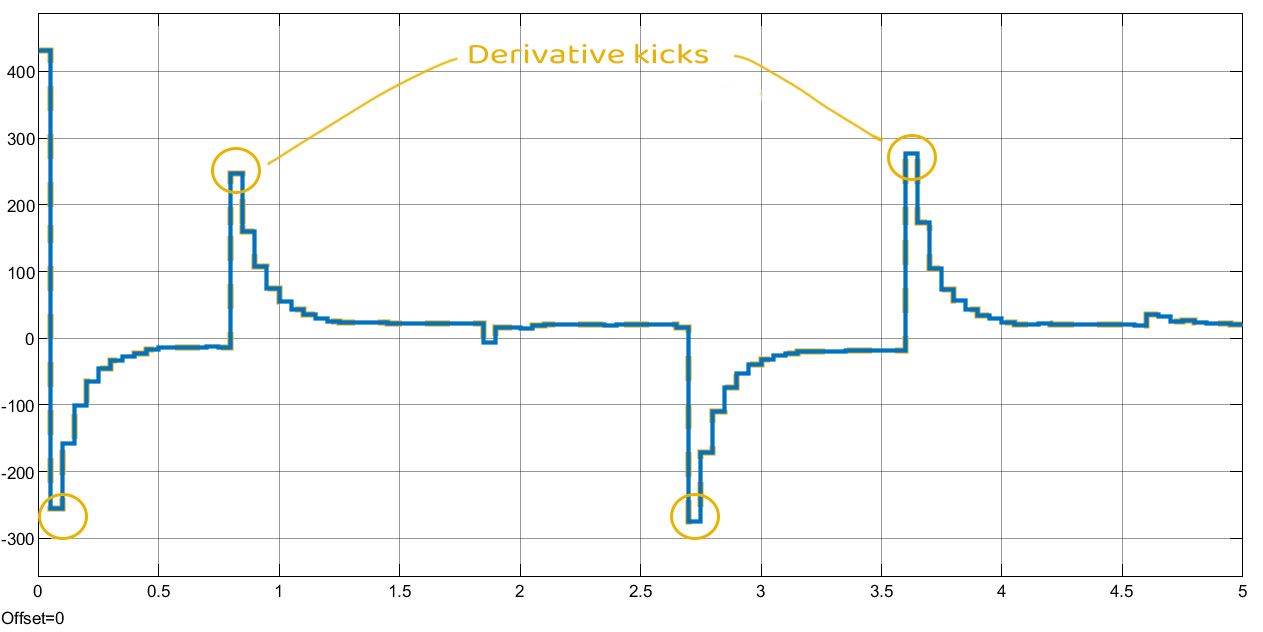
\includegraphics[width=0.75\linewidth]{Derivative_kicks.jpg}
    \caption{Illustratiion of the "Differential Kicks" Phenomenon }
    \label{fig:enter-label}
\end{figure}
To solve this issue an median filter was applied. This filter smoothed out the extreme and abrupt changes in the controller signal, ensuring a more controlled response. By computing the average controller signal over a 3 time window, this approach struck a balance between responsiveness and stability, enhancing the adaptability of the control system.
\end{onehalfspacing}


%Table 1 summarizes the tuned PID parameters obtained through manual tuning for each of the three PID controllers controlling the X and Y axes.

%\begin{table}[h]
%    \centering
%    \caption{Tuned PID Parameters for Real System Implementation}
%    \begin{tabular}{|c|c|c|c|}
%        \hline
%        & \text{Proportional Gain (\(K_P\))} & \text{Integral Gain (\(K_I\))} & \text{Derivative Gain (\(K_D\))} \\
%        \hline
%        \hline
%        PID X & 0.2 & 0.0005 & 0.1 \\
%        \hline
%        PID Y & 0.15 & 0.0003 & 0.08 \\
%        \hline
%    \end{tabular}
%\end{table}
